% ----------------------------------------------------------------------------
%                           FUNDAMENTAÇÃO TEÓRICA
% ----------------------------------------------------------------------------

\chapter{FUNDAMENTAÇÃO TEÓRICA}
\label{chap:fundamentacaoTeorica}

Este documento é um \emph{template} \LaTeX{} que foi concebido, primariamente, para ser utilizado na elaboração de Trabalho de Conclusão de Curso seguindo as normas da ABNT. Para isso, utilizamos a classe {\ttfamily abntex2.cls}.

Neste capítulo deve ser proporcionado o estado da arte / referencial teórico sobre o tema a que se refere o estudo. Um bom pesquisador não deve repetir trabalhos já concluídos ou que já estão em andamento. Por isso esta sessão é onde o autor demonstra até onde vai a pesquisa atual no campo de estudos em questão e estabelece as bases sobre as quais desenvolverá o estudo proposto.

Neste capítulo também são abordados detalhadamente os comandos para formatar o texto, criar listas, tabelas e figuras, inserir equações matemáticas, gerenciar referências bibliográficas.

% ----------------------------------------------------------------------------
%                                FORMATAÇÃO DE TEXTO
% ----------------------------------------------------------------------------
\section{Formatação de Texto}
\label{sec:formatacaoTexto}

\begin{itemize}
    \item \textbf{Negrito e Itálico:} Utilize os comandos \verb|\textbf{}| para negrito e \verb|\textit{}| para itálico. Exemplo: \textbf{texto em negrito} e \textit{texto em itálico}.
    
    \item \textbf{Aspas}: A palavra deve estar entre ``aspas simples duplas''.
    
    \item \textbf{Alinhamento do Texto:} Use \verb|\centering| para centralizar o texto, \verb|\raggedright| para alinhar à esquerda e \verb|\raggedleft| para alinhar à direita.
    
    \item \textbf{Parágrafos e Espaçamento:} Para criar novos parágrafos, deixe uma linha em branco.
    
    \item \textbf{Recuo de Parágrafo:} Se desejar evitar o recuo em um novo parágrafo, utilize o comando \verb|\noindent| no início.
    
    \item \textbf{Quebras de Linha e Página:} Para quebrar linhas, utilize \verb|\\| e \verb|\newline|. Para quebrar páginas, utilize \verb|\newpage|.
    
    \item \textbf{Comentários:} Utilize \verb|%| para fazer comentários no código LaTeX. Para comentários longos utilize  \verb|\begin{comment} ... \end{comment}|.
    % Você pode deixar comentários para quem for ler seu código ou para servir como suas anotações ao longo do texto.
    
    \item \textbf{Espaços:} Utilize \verb|~| para criar espaços não quebráveis.

\end{itemize}

% ----------------------------------------------------------------------------
%                                   LISTAS 
% ----------------------------------------------------------------------------
\section{Listas}
\label{sec:listas}

Em documentos \LaTeX, podemos criar listas não numeradas e numeradas utilizando os ambientes \verb|itemize| e \verb|enumerate|, respectivamente.

\subsection{Listas não numeradas}
\label{subsec:listasNaoNumeradas}
\noindent
Para criar listas não numeradas, use o ambiente \verb|itemize| e marque cada item com \verb|\item|.

\input{./dados/quadros/quadro2}

\subsection{Listas numeradas}
\label{subsec:listasNumeradas}
\noindent
Para criar listas numeradas, use o ambiente \verb|enumerate| e marque cada item com \verb|\item|.

\input{./dados/quadros/quadro3}

% ----------------------------------------------------------------------------
%                                   CITAÇÕES 
% ----------------------------------------------------------------------------
\section{Citações}
\label{sec:citacoes}

Nesta seção, vamos abordar como fazer citações diretas e indiretas utilizando os comandos \LaTeX{} apropriados.

\subsection{Citação indireta}
\label{subsec:citacaoIndireta}

A citação indireta é a transcrição das ideias de um autor, utilizando suas próprias palavras, mas mantendo o sentido original. Para fazer uma citação indireta, utilize os comandos \verb|\cite{chave}| e \verb|\citeonline{chave}|, colocando entre as chaves o nome do autor ou o identificador da referência bibliográfica.

\textbf{Exemplos:}
\begin{itemize}
    \item  Uma compreensão física é uma coisa completamente não-matemática, imprecisa e inexata, mas absolutamente necessária para um físico \cite{feynman}.
    \item Para \citeonline{feynman}, os físicos precisam ter flexibilidade para olhar os problemas sob diversos pontos de vista.
\end{itemize}

\subsection{Citação direta}
\label{subsec:citacaoDireta}

Quando o trecho citado é longo (4 ou mais linhas) deve-se usar um parágrafo específico para a citação, na forma de um texto recuado (4 cm da margem esquerda), com tamanho de letra menor e espaçamento entrelinhas simples. Exemplo de citação longa:
\\
\begin{citacao}
    Para qualquer campo eletrostático, não existe nenhum ponto de equilíbrio estável – exceto exatamente sobre uma outra carga. Usando a lei de Gauss, é fácil ver a razão disto. Primeiro, para uma carga estar em equilíbrio em qualquer ponto particular $P_0$, o campo ali deve ser zero. Segundo, para que este equilíbrio seja estável, devemos exigir que, se afastarmos a carga de $P_0$ em qualquer direção, surja uma força restauradora direcionada em oposição ao deslocamento. O campo elétrico em todos os pontos vizinhos deve apontar na direção de $P_0$. Mas, como podemos ver facilmente, se não existir nenhuma carga em $P_0$ isto é uma violação da lei de Gauss \cite[p.~51]{feynman}.

   % Desse modo, opera-se uma ruptura decisiva entre a reflexividade filosófica, isto é a possibilidade do sujeito de pensar e de refletir, e a objetividade científica. Encontramo-nos num ponto em que o conhecimento científico está sem consciência. Sem consciência moral, sem consciência reflexiva e também subjetiva. Cada vez mais o desenvolvimento extraordinário do conhecimento científico vai tornar menos praticável a própria possibilidade de reflexão do sujeito sobre a sua pesquisa \cite[p.~28]{Silva2000}.
\end{citacao}
\noindent
Para fazer a citação longa deve-se utilizar os seguintes comandos:
\begin{verbatim}
    \begin{citacao}
    <texto da citacao>
    \end{citacao}
\end{verbatim}

No exemplo acima, para a chamada da referência o comando \verb|\cite[p.~28]{Silva2000}| foi utilizado, visto que os nomes dos autores não são parte do trecho citado. É necessário também indicar o número da página da obra citada que contém o trecho citado.

\subsection{Citação Artigos de Mesmo Autor e Ano}
Quando houver dois artigos do mesmo autor publicados no mesmo ano, o LaTeX realiza a diferenciação automática nas citações, utilizando a notação \cite{lewis2018a, lewis2018b}. No entanto, essa diferenciação não ocorre automaticamente nas referências bibliográficas. Para incluir essa distinção nas referências, você deve adicionar a letra correspondente ao artigo no campo 'year' do arquivo .bib. Por exemplo, para dois artigos de 2018, você deve especificar "2018a" e "2018b" nos registros apropriados.

% ----------------------------------------------------------------------------
%                              REFERÊNCIAS CRUZADAS
% ----------------------------------------------------------------------------
\section{Referências Cruzadas}
\label{sec:referenciasCruzadas}

As referências cruzadas são uma funcionalidade essencial no \LaTeX{}, permitindo criar conexões automáticas entre diferentes partes do documento, como capítulos, seções, figuras, tabelas, equações e outros elementos numerados. Para utilizar referências cruzadas, é necessário incluir um rótulo ({\ttfamily label}) em cada elemento que se deseja referenciar.

\subsection{Inserindo um Rótulo}
Para criar um rótulo, utilize o comando \verb|\label{nome}| no local desejado. O \verb|nome| é um identificador único que você atribui ao elemento. É recomendável utilizar nomes descritivos, como \verb|chap:introducao| para um capítulo ou \verb|fig:exemplo| para uma figura. 

\textbf{Exemplo:}
\begin{verbatim}
    \section{Listas}
    \label{sec:listas}
\end{verbatim}

\subsection{Referenciando um Elemento}
Para fazer referência a um elemento previamente rotulado, utilize os comandos \verb|\ref{nome}|, \verb|\autoref{nome}| ou \verb|\cref{nome}|. O comando \verb|\ref{nome}| simplesmente mostra o número do elemento referenciado, o comando \verb|\autoref{nome}| adiciona automaticamente o tipo do elemento (como ``Capítulo'', ``Figura'', ``Equação'', etc.) antes do número, enquanto \verb|\cref{nome}| é similar ao comando anterior, mas o tipo do elemento é abreviado (como ``Cap.'', ``Fig.'', ``Eq.'', etc.).

\textbf{Exemplo:}
\begin{verbatim}
    Na \autoref{sec:listas} são abordadas informações sobre listas no documento.
\end{verbatim}

\textbf{Resultado:} \\
``Na \autoref{sec:listas} são abordadas informações sobre listas no documento.''

\subsection{Elementos com rótulos}
Aqui estão alguns elementos comuns que podem receber rótulos para referências cruzadas:
\begin{itemize}
    \item Capítulos: \texttt{\textbackslash chapter\{...\}\textbackslash label\{chap:nome\}}
    \item Seções: \texttt{\textbackslash section\{...\}\textbackslash label\{sec:nome\}}
    \item Subseções: \texttt{\textbackslash subsection\{...\}\textbackslash label\{subsec:nome\}}
    \item Figuras: \texttt{\textbackslash begin\{figure\}...\textbackslash caption\{...\}\textbackslash label\{fig:nome\}\textbackslash end\{figure\}}
    \item Tabelas: \texttt{\textbackslash begin\{table\}...\textbackslash caption\{...\}\textbackslash label\{tab:nome\}\textbackslash end\{table\}}
    \item Equações: \texttt{\textbackslash begin\{equation\}...\textbackslash label\{eq:nome\}\textbackslash end\{equation\}}
\end{itemize}
\vspace{0.5cm}
Com o uso adequado de rótulos e referências cruzadas, você pode criar um documento bem estruturado e de fácil navegação no \LaTeX{}. 

% ----------------------------------------------------------------------------
%                                   FIGURAS
% ----------------------------------------------------------------------------
\section{Figuras}
\label{sec:figuras}

Exemplo de como inserir a \autoref{fig:figura-exemplo-1}, que pode ser referenciado como \cref{fig:figura-exemplo-1}. As figuras aparecem automaticamente na lista de figuras. Os arquivos das imagens devem ser armazenados no diretório de ``/dados''.

\begin{figure}[!htb]
    \centering
    \caption{Possíveis distribuições de cargas de espessura não nula.}
    \sbox0{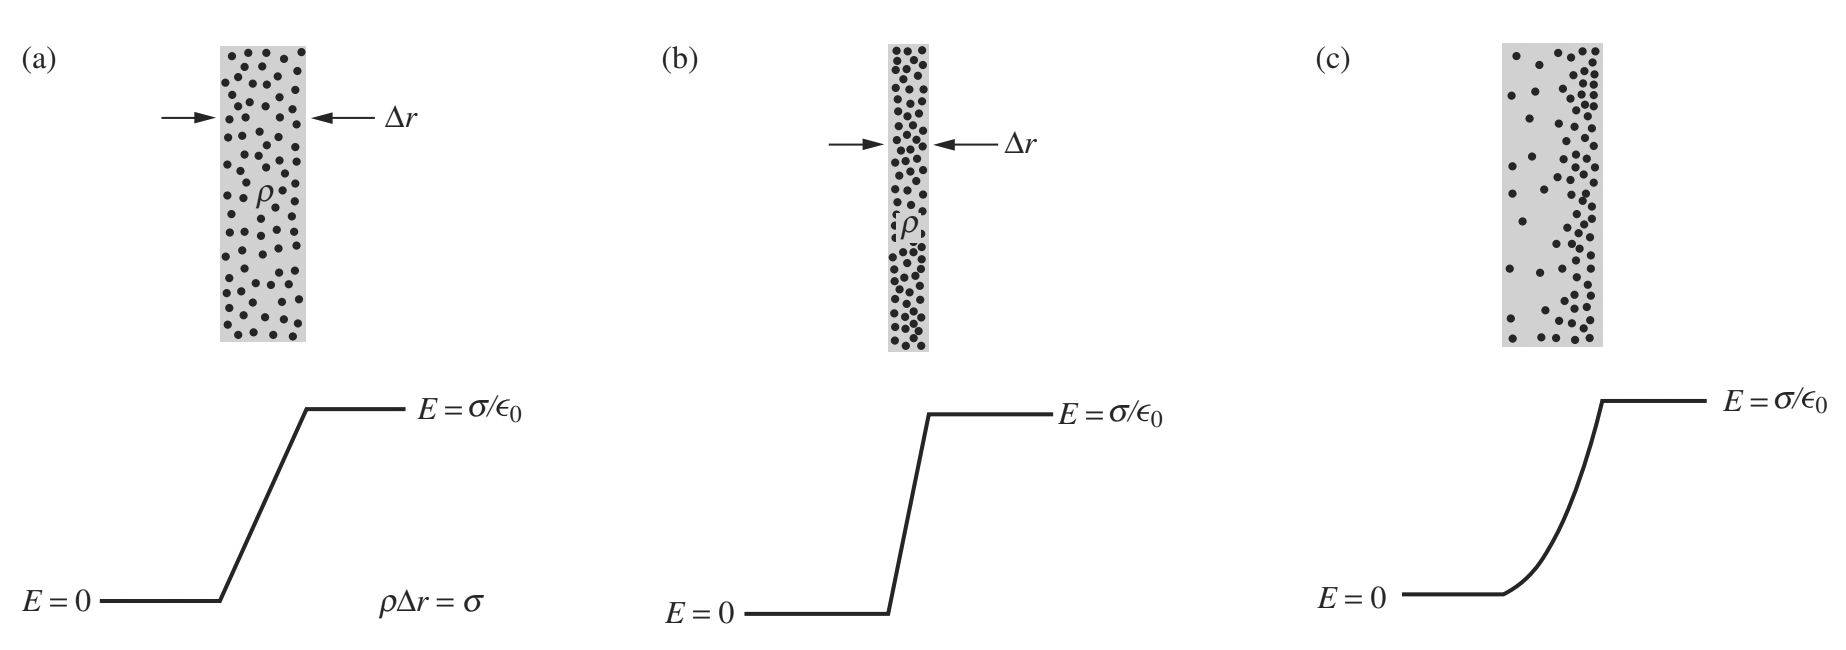
\includegraphics[width=0.8\textwidth]{./dados/figuras/purcell}}
    \begin{minipage}{\wd0}
        \usebox0
        \vspace{-20pt}
        \label{fig:figura-exemplo-1}
        \fonte{\citeonline[p.~31]{purcell}.}
    \end{minipage}
\end{figure}

% ----------------------------------------------------------------------------
%                                QUADROS E TABELAS
% ----------------------------------------------------------------------------
\section{Quadros e tabelas}
\label{sec:quadrosTabelas}

Exemplo de como inserir o \autoref{qua:quadro-exemplo1} e a \cref{tab:tabela-exemplo1}. Ambos aparecem automaticamente nas suas respectivas listas.
Os elementos (Quadros e Tabelas) devem ser criados em arquivos separados para facilitar manutenção e armazenados no diretório de ``/dados".

\input{./dados/quadros/quadro1}

A diferença entre quadro e tabela está no fato que um quadro é formado por linhas horizontais e verticais. Deve ser utilizado quando o conteúdo é majoritariamente não-numérico. Uma tabela é formada apenas por linhas verticais, e deve ser utilizada quando o conteúdo é majoritariamente numérico.

\input{./dados/tabelas/tabela1}

% ----------------------------------------------------------------------------
%                                  EQUAÇÕES
% ----------------------------------------------------------------------------
\section{Equações}
\label{sec:equacoes}

Exemplo de como inserir a \autoref{eq:equacao-exemplo1} e a \cref{eq:equacao-exemplo2} no corpo do texto. Observe que foram utilizadas duas formas distintas para referenciar as equações. O comando \verb|\ref{nome}| também é válido para exibir apenas o número da equação.

\begin{equation}
    \label{eq:equacao-exemplo1}
    f(x) = \frac{a_0}{2} + \sum_{n=1}^{\infty} \left[a_n \cos{ \left( \frac{ n\pi x}{L} \right) }  +  b_n  \: \mathrm{sen}{ \left( \frac{ n\pi x}{L} \right) }     \right]
    ,
\end{equation}

\begin{align}
    \phi_E  = \int \limits_{A} \Vec{E_1}\cdot (-\Hat{n}) \, dA'\ + \int \limits_{A} \Vec{E_2}\cdot \Hat{n} \, dA'\
    \label{eq:equacao-exemplo2}
\end{align}
\noindent
A numeração das equações é inserida e atualizada automaticamente. É possível remover o número de uma equação ao adicionar um asterisco no parâmetro  {\ttfamily equation}, como em

\begin{equation*}
    \oint \limits_S \Vec{E}\cdot d \Vec{A}\ =
    \frac{Q_{\mathrm{enc}}}{\varepsilon_0}
    .
\end{equation*}

Existem outros parâmetros para inserir equações, como o {\ttfamily align},  {\ttfamily split}.
Além disso, o ambiente matemático pode ser utilizado ao longo do texto ao envolver a equação com cifrão (\$). Por exemplo, como feito com a equação $ dE_x = dE \cos\theta $.

% ----------------------------------------------------------------------------
%                                   ALGORITMOS
% ----------------------------------------------------------------------------
\section{Algoritmos}
\label{sec:algoritmos}

Exemplo de como inserir um algoritmo. Para inserção de algoritmos utiliza-se o pacote {\ttfamily algorithm2e} que já está devidamente configurado dentro do template.
Os algoritmos devem ser criados em arquivos separados para facilitar manutenção e armazenados no diretório de ``/dados''. \\
\input{./dados/algoritmos/algoritmo1}

% ----------------------------------------------------------------------------
%                           REFERÊNCIAS BIBLIOGRÁFICAS
% ----------------------------------------------------------------------------
\section{Referências bibliográficas}
\label{sec:referenciasBibliograficas}

A bibliografia é feita no padrão \textsc{Bib}\TeX{}. Para facilitar a manutenção, as referências são colocadas em um arquivo separado. Neste \textit{template} as referências são armazenadas no arquivo \verb|base-referencias.bib|.

Existem diversas categorias documentos e materiais componentes da bibliografia. A classe abn\TeX{} define as seguintes categorias (entradas):

\begin{verbatim}
@book
@inbook
@article
@phdthesis
@mastersthesis
@monography
@techreport
@manual
@proceedings
@inproceedings
@journalpart
@booklet
@patent
@unpublished
@misc
\end{verbatim}

Cada categoria (entrada) é formatada pelo pacote \citeonline{abnTeX22014d} de uma forma específica. Algumas entradas foram introduzidas especificamente para atender à norma \citeonline{NBR6023:2002}, são elas: \verb|@monography|, \verb|@journalpart|, \verb|@patent|. As demais entradas são padrão \textsc{Bib}\TeX{}.
